\section{Results}
\label{sec:results}

\subsection{Which metrics respond to known delays}
\label{sec:res-metrics}

A timing metric should worsen steadily as a known delay grows and should rank a clip with the right kind of sound but unrelated timing as badly aligned. We delay each of 200 FlashDot development spectrograms by 2 to 64 mel frames (23 to 743\,ms), filling the start with the clip's quietest frame, and compare it with the original; as a second reference we compare each clip with a different clip (\cref{fig:sensitivity}; values in \cref{tab:sensitivity}).


\begin{figure}[t]
  \centering
  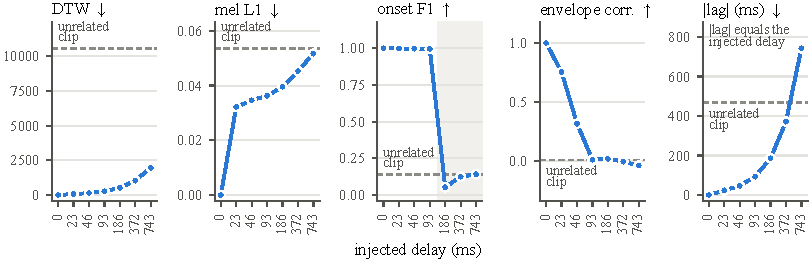
\includegraphics[width=\linewidth]{figures/metric_sensitivity.pdf}
  \caption{Metric response to injected delays on FlashDot (development, 200 clips). Dashed lines: an unrelated clip. Only $|$lag$|$ grows in proportion to the delay; DTW and mel L1 rank every delay as closer to the truth than an unrelated clip.}
  \label{fig:sensitivity}
\end{figure}

On FlashDot, where each delay is a pure shift of identical audio, the envelope lag recovers the injected delay exactly. Onset F1 is flat up to 93\,ms, inside its tolerance, and drops to the level of an unrelated clip (about 0.14) or below from 186\,ms. Envelope correlation falls from 0.75 at 23\,ms to about zero by 93\,ms, so it cannot tell 100\,ms from a second. DTW grows with delay, from 69 at 23\,ms to 1968 at 743\,ms, but an unrelated clip scores 10582: a large delay looks five times closer to the truth than a clip with different content. This is expected, since DTW tolerates time shifts by construction, and it makes DTW unsuited as a timing metric. Mel L1 jumps at the smallest delay and then barely separates a 743\,ms delay (0.052) from an unrelated clip (0.054). We therefore use $|$lag$|$, within-one-frame, onset F1 and, on FlashDot, tone F1 as timing metrics, and leave DTW out. These delays are exact shifts of identical audio, so the check shows how each metric responds to a pure delay and does not establish how well it tracks timing errors in generated audio.

\subsection{PAL as a training loss does not improve timing}
\label{sec:res-loss}

% Generated by perceptalign/paper_tables.py; do not edit by hand (sources: paper/generated/sources.md).
\providecommand{\std}[1]{\,{\scriptsize$\pm$#1}}
\begin{table}[t]
  \centering
  \caption{FlashDot. Top: references. Middle: PAL as a loss and the CE baselines, trained from scratch (development split, 2000 steps unless stated). Bottom: PAL as a reward. Sync acc.\ is the held-out critic at tolerance 1 (chance $\approx 0.14$); within 1 frame is the share of clips with $|$lag$|$ within one video frame. Mean $\pm$ std over three training seeds; $^{\dagger}$\,single training seed. Best of 8 on the development split uses training seed 0.}
  \label{tab:flashdot}
  \small
  \begin{tabular}{llcccc}
    \toprule
    Model & Split & Tone F1 $\uparrow$ & $|$Lag$|$ (ms) $\downarrow$ & Within 1 frame $\uparrow$ & Sync acc.\ $\uparrow$ \\
    \midrule
    VQGAN reconstruction                                 & dev  & 0.970 & 2.7 & 1.000 & 1.000 \\
    VQGAN reconstruction                                 & test & 0.971 & 4.9 & 0.995 & 1.000 \\
    \midrule
    CE (teacher forcing)                                 & dev  & 0.414\std{0.007} & 410\std{14} & 0.108\std{0.020} & 0.200\std{0.030} \\
    CE, corrupted prefix ($p_{\mathrm{keep}} = 0.5$)     & dev  & 0.501\std{0.028} & 317\std{15} & 0.190\std{0.017} & 0.267\std{0.033} \\
    CE + PAL, teacher-forced (3000 steps)                & dev  & 0.315\std{0.016} & 485\std{26} & 0.050\std{0.015} & 0.112\std{0.033} \\
    CE + PAL, half-corrupted PAL prefix                  & dev  & 0.255\std{0.024} & 502\std{24} & 0.055\std{0.020} & 0.117\std{0.006} \\
    CE + PAL, fully corrupted PAL prefix$^{\dagger}$     & dev  & 0.279 & 491 & 0.060 & 0.125 \\
    \midrule
    CE, corrupted prefix, best of 8$^{\dagger}$          & dev  & 0.535 & 228 & 0.480 & 0.645 \\
    \midrule
    CE, corrupted prefix                                 & test & 0.498\std{0.014} & 340\std{12} & 0.198\std{0.016} & 0.233\std{0.016} \\
    \quad best of 8                                      & test & 0.567\std{0.027} & 239\std{14} & 0.422\std{0.026} & 0.705\std{0.031} \\
    \quad self-training, random selection                & test & 0.449\std{0.012} & 384\std{21} & 0.128\std{0.033} & 0.178\std{0.033} \\
    \quad self-training, PAL selection                   & test & 0.458\std{0.029} & 359\std{24} & 0.133\std{0.010} & 0.185\std{0.020} \\
    \bottomrule
  \end{tabular}
\end{table}


On FlashDot, every way of adding PAL to the loss lowers timing quality (\cref{tab:flashdot}, middle; means over three training seeds on the development split, except for the fully corrupted row, which is one seed). With teacher-forced logits, tone F1 falls from 0.414 to 0.315 and held-out sync accuracy (tolerance 1) from 0.200 to 0.112, below chance (about 0.14), even with 1000 more training steps. Computing PAL from a half or fully corrupted prefix, so that the video is the only source of timing, does no better (tone F1 0.255 and 0.279). Corrupting the prefix of the cross-entropy pass alone, with no critic, helps instead: tone F1 0.501, $|$lag$|$ 317\,ms. The two diagnostics of \cref{sec:diagnostics} are consistent with the shortcut account below. They do not exclude other causes of the drop, such as the single loss weight ($\beta = 1$) or interference between the two gradients.

\paragraph{Exposure bias.}
The CE model does use the video under teacher forcing: over the 200 development clips, and as a mean over three training seeds, development cross-entropy is 1.54 with each clip's own visual features and 1.89 with another clip's. With a fully corrupted prefix it is 4.51 against 4.66, close to the uniform level of 4.85, so the video alone tells the model little about which code comes next. This suggests that teacher-forced predictions inherit their timing from the aligned prefix and look aligned to the critic whatever the model does with the video, while the model's free-running samples have low timing accuracy (held-out sync accuracy 0.200 at tolerance 1, against a chance level of about 0.14). A PAL gradient on teacher-forced logits would then reward copying the prefix, which the model already does.

\paragraph{The critic can be exploited.}
Corrupting the PAL prefix removes the shortcut through the prefix but opens another one. In the free-logit attack (\cref{fig:attack}), optimizing logits directly against the mel critic reaches a PAL of 0.98, about that of the ground-truth codes (0.95; random codes 2.12). The decoded spectrograms are broadband texture with tone F1 0.28, barely above random codes (0.20) and far from the ground truth (0.98). Critics that see only 8, 4 or 1 band energies are fooled the same way. Coarser critics do align energy changes better at the optimum, with $|$lag$|$ of 151\,ms (mel), 147\,ms (8 bands), 48\,ms (4 bands) and 15\,ms (1 band) against 644\,ms for random codes, but none of them produces the tone: tone F1 at the optimum is 0.28, 0.28, 0.11 and 0.05. A critic trained only on real audio has not seen spectrograms like these, which is a likely reason it scores them as aligned.

\begin{figure}[t]
  \centering
  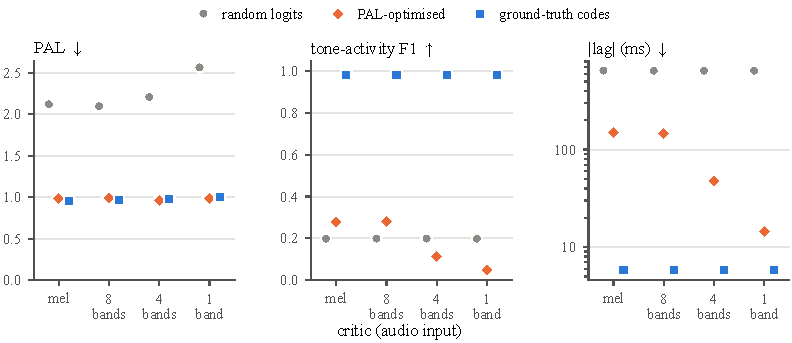
\includegraphics[width=\linewidth]{figures/critic_attack.pdf}
  \caption{Free-logit attack on four FlashDot critics (eight development clips). Optimizing logits against PAL (orange) reaches the PAL of the ground-truth codes (blue) for every critic, while tone F1 stays far below the ground truth (0.98): 0.28 for the mel and 8-band critics against 0.20 for random codes (grey), and lower for the 4-band and 1-band critics. Coarser critics bring the envelope lag down, but none recovers the tone.}
  \label{fig:attack}
\end{figure}

\subsection{PAL as a reward on samples}
\label{sec:res-reward}

Used to choose among the generator's own samples, the same critic helps. Keeping the best of eight free-running samples from the corruption-trained CE model (candidates scored with $\sigma = 0$) raises tone F1 from 0.499 to 0.535, the share of clips within one video frame from 0.17 to 0.48, and held-out sync accuracy (tolerance 1) from 0.245 to 0.645 on the FlashDot development split (training seed 0) (\cref{tab:flashdot}). The tone F1 gain is modest; the larger held-out gain partly reflects that the two critics share features and model family. \Cref{fig:fd-samples} shows one development clip: the clip whose $|$lag$|$ gain from re-ranking is the median over clips, so it shows a typical case rather than the best one.

\begin{figure}[t]
  \centering
  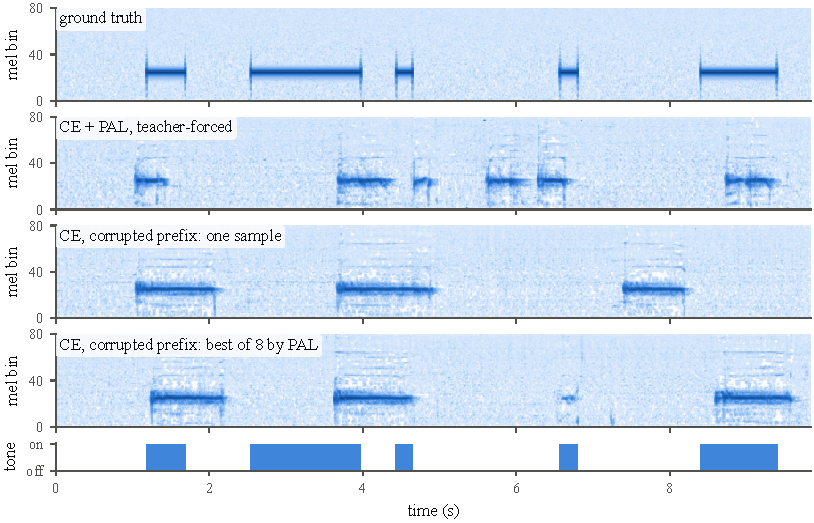
\includegraphics[width=\linewidth]{figures/flashdot_samples.pdf}
  \caption{One FlashDot development clip (the clip with the median $|$lag$|$ gain from best-of-8 re-ranking). The bottom row marks when the tone is on. The model trained with PAL as a loss (teacher-forced) adds tones that are not in the video; the corruption-trained CE model misses some tones; keeping the best of eight of its samples by PAL matches more of the tones (tone F1 0.57 on this clip, against 0.33 for the single sample), though its lag is still large (790\,ms against 859\,ms).}
  \label{fig:fd-samples}
\end{figure}

On the FlashDot test split, over three generator seeds and with candidates scored at $\sigma = 1$ (the setting used for VAS and for self-training), best-of-8 re-ranking raises tone F1 from 0.498 to 0.567, the share of clips within one frame from 0.20 to 0.42, and held-out sync accuracy (tolerance 1) from 0.23 to 0.71 (means over seeds). Seeds are the unit of replication, so we report each seed. Against one sample, best of 8 raises tone F1 by 0.054 ($p = 0.001$), 0.084 and 0.068 (both $p < 0.001$) and the share of clips within one frame by 0.205, 0.195 and 0.270 (all $p < 0.001$); the sign is the same in every seed. The oracle that keeps the candidate with the best true tone F1 reaches only 0.39 held-out sync accuracy against 0.71 for PAL selection (\cref{tab:window}), so the held-out score partly measures agreement with the selecting critic; tone F1 and the within-one-frame share are the primary timing measures.

Self-training does not keep this gain. After two rounds (400 clips per round, eight candidates, 300 steps), mean tone F1 falls to 0.458 with PAL selection and 0.449 with random selection, below the 0.498 of the starting model, and the share of clips within one frame falls from 0.20 to 0.13 with either rule. Per seed (0, 1, 2), the change in tone F1 against the starting model is $-0.010$ ($p = 0.47$), $-0.052$ and $-0.059$ (both $p < 0.001$) with PAL selection and $-0.043$ ($p = 0.002$), $-0.056$ and $-0.050$ (both $p < 0.001$) with random selection. PAL minus random selection is $+0.033$ ($p = 0.01$), $+0.004$ ($p = 0.75$) and $-0.008$ ($p = 0.54$) in tone F1, so the selection rule does not matter consistently. Because fine-tuning on the model's own samples lowered tone F1 with either selection rule, the FlashDot self-training arms say little about the critic's choice; the ground-truth-only control exists only on VAS.

% Generated by perceptalign/paper_tables.py; do not edit by hand (sources: paper/generated/sources.md).
\providecommand{\stackstd}[2]{\begin{tabular}[t]{@{}c@{}}#1\\[-2pt]{\scriptsize #2}\end{tabular}}
\begin{table}[t]
  \centering
  \caption{VAS test results (768 clips of the SpecVQGAN \texttt{vas\_valid} list), one sample per clip unless stated. Sync acc.\ is the held-out critic at tolerance 0 / 1 (chance $\approx 0.05$ / $0.14$). On.: onset; Env.: envelope correlation; $|$Lag$|$ in ms; 1 fr.: share of clips with $|$lag$|$ within one video frame. Fine-tuned rows train LoRA adapters with the same budget.}
  \label{tab:vas}
  \small
  \setlength{\tabcolsep}{3.2pt}
  \begin{tabular}{lcccccccc}
    \toprule
    Model & On.\ F1 $\uparrow$ & On.\ AP $\uparrow$ & Env.\ $\uparrow$ & $|$Lag$|$ $\downarrow$ & 1 fr.\ $\uparrow$ & Sync acc.\ $\uparrow$ & FID $\downarrow$ & MKL $\downarrow$ \\
    \midrule
    Ground truth                 & -- & -- & -- & -- & -- & 0.285 / 0.536 & -- & -- \\
    VQGAN reconstruction         & 0.813 & 0.778 & 0.918 & 0.2 & 100\% & 0.277 / 0.518 & 6.0 & 1.03 \\
    \midrule
    Pretrained SpecVQGAN         & 0.368 & 0.206 & 0.003 & 502 & 5.6\% & 0.061 / 0.167 & 27.8 & 5.81 \\
    \quad best of 4              & 0.376 & 0.215 & 0.015 & 456 & 6.6\% & 0.151 / 0.375 & 26.7 & 5.92 \\
    \quad GT-only fine-tune      & \placeholder{} & \placeholder{} & \placeholder{} & \placeholder{} & \placeholder{} & \placeholder{} / \placeholder{} & \placeholder{} & \placeholder{} \\
    \quad self-train, random     & \placeholder{} & \placeholder{} & \placeholder{} & \placeholder{} & \placeholder{} & \placeholder{} / \placeholder{} & \placeholder{} & \placeholder{} \\
    \quad self-train, PAL        & \placeholder{} & \placeholder{} & \placeholder{} & \placeholder{} & \placeholder{} & \placeholder{} / \placeholder{} & \placeholder{} & \placeholder{} \\
    \bottomrule
  \end{tabular}
\end{table}


On VAS (\cref{tab:vas}), the VQGAN reconstruction reaches FID 6.0 and MKL 1.03, matching the published codebook numbers (6.0 and 1.0), which checks our port of the evaluation. The pretrained SpecVQGAN transformer (top-$k$ 100, one sample per clip) gives FID 27.8 and MKL 5.81 (published 25.4 and 5.9). Its timing is close to chance: envelope correlation 0.003, $|$lag$|$ 502\,ms, 5.6\% of clips within one frame, and held-out sync accuracy at tolerance 0 / 1 of 0.061 / 0.167, against chance levels of about 0.05 / 0.14. The ground truth itself reaches only 0.285 / 0.536 (tolerance 0 / 1) under the held-out critic, which bounds what that metric can show. 

Keeping the best of four samples per clip by PAL improves the timing measures that follow the envelope: $|$lag$|$ falls by 46\,ms (95\% interval 16 to 74\,ms, $p = 0.002$, paired bootstrap over the 768 clips), envelope correlation rises from 0.003 to 0.015 ($p < 0.001$) and held-out sync accuracy at tolerance 1 from 0.167 to 0.375, at four times the sampling cost. Onset F1 ($+0.008$, $p = 0.10$) does not change significantly, and the share of clips within one frame stays at 5.6 to 6.6\% ($p = 0.41$), and FID and MKL stay close to the single-sample values. The held-out gain is the largest, and it is the one most open to shared bias between the two critics (\cref{sec:limitations}).

Self-training does not carry this gain into the generator. With the same LoRA budget (two rounds of 256 clips, four candidates, 150 steps each), self-training with PAL selection, self-training with random selection and fine-tuning on ground truth alone give the same timing: no two of the three differ significantly on any timing measure (all $p > 0.1$). For PAL against random selection, onset F1 differs by $+0.003$ ($p = 0.50$), $|$lag$|$ by $+22$\,ms ($p = 0.13$) and sync accuracy at tolerance 1 by $+0.001$ ($p = 0.98$). All three lower onset F1 by about 0.02 against the pretrained model ($p < 0.001$), and only random selection lowers $|$lag$|$ significantly ($-35$\,ms, $p = 0.01$). All three also lower FID, and ground-truth-only fine-tuning lowers it most (20.4, against 24.1 with PAL selection and 25.1 with random selection). On VAS this suggests that the FID gain comes from fine-tuning on in-domain audio (FID values are single runs), and at this budget PAL selection adds nothing measurable to timing or quality.

% Generated by perceptalign/paper_tables.py; do not edit by hand (sources: paper/generated/sources.md).
\providecommand{\std}[1]{\,{\scriptsize$\pm$#1}}
\begin{table}[t]
  \centering
  \caption{Candidate selection on the test split: every row chooses among the same 8 free-running samples per clip. FlashDot: corruption-trained CE generator, \placeholder{} clips, mean $\pm$ std over \placeholder{} generator seeds. VAS: pretrained SpecVQGAN, \placeholder{} clips, one run. $\sigma$: width of the binding window on the audio-early side, $\sigma_{\mathrm{late}}$ on the audio-late side (\cref{eq:window}). Sync: held-out critic at tolerance 1. The oracle keeps the candidate with the best true tone F1 (FlashDot) or smallest $|$lag$|$ (VAS).}
  \label{tab:window}
  \small
  \setlength{\tabcolsep}{3.2pt}
  \begin{tabular}{lccccccc}
    \toprule
    & \multicolumn{3}{c}{FlashDot} & \multicolumn{4}{c}{VAS} \\
    \cmidrule(lr){2-4} \cmidrule(lr){5-8}
    Selection & Tone F1 $\uparrow$ & 1 fr.\ $\uparrow$ & Sync $\uparrow$ & 1 fr.\ $\uparrow$ & $|$Lag$|$ $\downarrow$ & Sync $\uparrow$ & FID $\downarrow$ \\
    \midrule
    One sample                                           & \placeholder{} & \placeholder{} & \placeholder{} & \placeholder{} & \placeholder{} & \placeholder{} & \placeholder{} \\
    Best of 8, $\sigma = 0$                              & \placeholder{} & \placeholder{} & \placeholder{} & \placeholder{} & \placeholder{} & \placeholder{} & \placeholder{} \\
    Best of 8, $\sigma = 0.5$                            & \placeholder{} & \placeholder{} & \placeholder{} & \placeholder{} & \placeholder{} & \placeholder{} & \placeholder{} \\
    Best of 8, $\sigma = 1$                              & \placeholder{} & \placeholder{} & \placeholder{} & \placeholder{} & \placeholder{} & \placeholder{} & \placeholder{} \\
    Best of 8, $\sigma = 2$                              & \placeholder{} & \placeholder{} & \placeholder{} & \placeholder{} & \placeholder{} & \placeholder{} & \placeholder{} \\
    Best of 8, $\sigma = 0.5$, $\sigma_{\mathrm{late}} = 2$ & \placeholder{} & \placeholder{} & \placeholder{} & \placeholder{} & \placeholder{} & \placeholder{} & \placeholder{} \\
    Best of 8, $\sigma = 2$, $\sigma_{\mathrm{late}} = 0.5$ & \placeholder{} & \placeholder{} & \placeholder{} & \placeholder{} & \placeholder{} & \placeholder{} & \placeholder{} \\
    \midrule
    Oracle (upper bound)                                 & \placeholder{} & \placeholder{} & \placeholder{} & \placeholder{} & \placeholder{} & \placeholder{} & \placeholder{} \\
    \bottomrule
  \end{tabular}
\end{table}


\paragraph{Binding window.} \Cref{tab:window} scores the same eight candidates per clip under different windows. Every window improves on one sample. Tone F1 barely depends on the window (0.551 to 0.572 on FlashDot), while the other measures trade off: the within-one-frame share ranges from 0.370 to 0.463 and held-out sync accuracy from 0.590 to 0.705. On FlashDot the narrowest window ($\sigma = 0$, exact zero offset) puts more clips within one frame than $\sigma = 1$ in all three seeds (0.463 against 0.422 on average), but the difference is significant only in seed 0 ($p = 0.01$; $p = 0.36$ and $0.40$ in the others). In turn, $\sigma = 1$ gives higher held-out sync accuracy at tolerance 1, the tolerance that window matches, in all three seeds (0.705 against 0.590, $p < 0.001$ in each) and higher onset F1 in all three ($p \le 0.014$). On VAS (one run, 256 clips), $\sigma = 0$ and $\sigma = 1$ do not differ significantly on any measure. Neither asymmetric window gives a consistent gain over the symmetric $\sigma = 1$ window, and the window with a wide audio-late side ($\sigma = 0.5$, $\sigma_{\mathrm{late}} = 2$) lowers held-out sync accuracy relative to $\sigma = 1$ on FlashDot in all three seeds ($p \le 0.009$) and on VAS ($-0.066$, $p = 0.003$). The oracle rows show how far any PAL choice is from the best available candidate: on VAS, choosing by true lag puts 40\% of clips within one frame, against 7 to 9\% for every PAL window.

\section{Discussion}
\label{sec:discussion}

The same frozen critic hurts timing as a loss and helps as a selector at sampling time, and the two diagnostics are consistent with one account of the difference. A differentiable loss scores whatever the gradient path produces: under teacher forcing that is a prediction already aligned by its prefix, and with the prefix removed it is a point the generator can move toward freely, including spectrograms outside anything the critic was trained on. A reward on free-running samples scores only what the generator actually produces, so the critic works inside the region where its ranking means something. That ranking did not carry over into the generator's weights: fine-tuning on the critic's choices matched fine-tuning on random choices on both datasets, and on FlashDot both fell below the starting model. The gain from selection is specific to each clip and its video, and two short rounds of cross-entropy on a few hundred chosen samples did not teach the generator to make such choices itself; larger budgets or a training signal that compares candidates directly may behave differently. This matches what is known about optimizing learned rewards \citep{gao2023scaling}: the less freely the optimizer can move against the reward model, the more the reward keeps its meaning. For similar setups, we suggest running the wrong-video probe and the free-logit attack before training against a critic, and using the critic to select samples at generation time. Our results give no support to the perceptual motivation for the window: no window is best on every measure, and the asymmetric windows that follow the human tolerance for late audio bring no gain. We keep the window as a parameter of PAL rather than as a claim about perception.
